% ------------------------------------------------------------
% LaTeX Template für die DHBW zum Schnellstart!
% Original: https://github.wdf.sap.corp/vtgermany/LaTeX-Template-DHBW
% ------------------------------------------------------------
% ---- Präambel mit Angaben zum Dokument
\documentclass[
	fontsize=12pt,           % Leitlinien sprechen von Schriftgröße 12.
	paper=A4,
	twoside=false,
	listof=totoc,            % Tabellen- und Abbildungsverzeichnis ins Inhaltsverzeichnis
	bibliography=totoc,      % Literaturverzeichnis ins Inhaltsverzeichnis aufnehmen
	titlepage,               % Titlepage-Umgebung anstatt \maketitle
	headsepline,             % horizontale Linie unter Kolumnentitel
	abstract,              % Überschrift einschalten, Abstract muss in {abstract}-Umgebung stehen
]{scrreprt}                  % Verwendung von KOMA-Report
\usepackage[utf8]{inputenc}  % UTF8 Encoding einschalten
\usepackage[ngerman]{babel}  % Neue deutsche Rechtschreibung
\usepackage[T1]{fontenc}     % Ausgabe von westeuropäischen Zeichen (auch Umlaute)
\usepackage{microtype}       % Trennung von Wörtern wird besser umgesetzt
\usepackage{lmodern}         % Nicht-gerasterte Schriftarten (bei MikTeX erforderlich)
\usepackage{graphicx}        % Einbinden von Grafiken erlauben
\usepackage{wrapfig}         % Grafiken fließend im Text
\usepackage{setspace}        % Zeilenabstand \singlespacing, \onehalfspaceing, \doublespacing
\usepackage[
	%showframe,                % Ränder anzeigen lassen
	left=2.7cm, right=2.5cm,
	top=2.5cm,  bottom=2.5cm,
	includeheadfoot
]{geometry}                      % Seitenlayout einstellen
\usepackage{scrlayer-scrpage}    % Gestaltung von Fuß- und Kopfzeilen
\usepackage{acronym}             % Abkürzungen, Abkürzungsverzeichnis
\usepackage{titletoc}            % Anpassungen am Inhaltsverzeichnis
\contentsmargin{0.75cm}          % Abstand im Inhaltsverzeichnis zw. Punkt und Seitenzahl
\usepackage[                     % Klickbare Links (enth. auch "nameref", "url" Package)
  hidelinks,                     % Blende die "URL Boxen" aus.
  breaklinks=true                % Breche zu lange URLs am Zeilenende um
]{hyperref}
\usepackage[hypcap=true]{caption}% Anker Anpassung für Referenzen
\urlstyle{same}                  % Aktuelle Schrift auch für URLs
% Anpassung von autoref für Gleichungen (ergänzt runde Klammern) und Algorithm.
% Anstatt "Listing" kann auch z.B. "Code-Ausschnitt" verwendet werden. Dies sollte
% jedoch synchron gehalten werden mit \lstlistingname (siehe weiter unten).
\addto\extrasngerman{%
	\def\equationautorefname~#1\null{Gleichung~(#1)\null}
	\def\lstnumberautorefname{Zeile}
	\def\lstlistingautorefname{Listing}
	\def\algorithmautorefname{Algorithmus}
	% Damit einheitlich "Abschnitt 1.2[.3]" verwendet wird und nicht "Unterabschnitt 1.2.3"
	% \def\subsectionautorefname{Abschnitt}
}

% ---- Abstand verkleinern von der Überschrift 
\renewcommand*{\chapterheadstartvskip}{\vspace*{.5\baselineskip}}

% Hierdurch werden Schusterjungen und Hurenkinder vermieden, d.h. einzelne Wörter
% auf der nächsten Seite oder in einer einzigen Zeile.
% LaTeX kann diese dennoch erzeugen, falls das Layout ansonsten nicht umsetzbar ist.
% Diese Werte sind aber gute Startwerte.
\widowpenalty10000
\clubpenalty10000

% ---- Für das Quellenverzeichnis
\usepackage[
	backend = biber,                % Verweis auf biber
	language = auto,
	style = numeric,                % Nummerierung der Quellen mit Zahlen
	sorting = none,                 % none = Sortierung nach der Erscheinung im Dokument
	sortcites = true,               % Sortiert die Quellen innerhalb eines cite-Befehls
	block = space,                  % Extra Leerzeichen zwischen Blocks
	hyperref = true,                % Links sind klickbar auch in der Quelle
	%backref = true,                % Referenz, auf den Text an die zitierte Stelle
	bibencoding = auto,
	giveninits = true,              % Vornamen werden abgekürzt
	doi=false,                      % DOI nicht anzeigen
	isbn=false,                     % ISBN nicht anzeigen
    alldates=short                  % Datum immer als DD.MM.YYYY anzeigen
]{biblatex}
\addbibresource{Inhalt/literatur.bib}
\setcounter{biburlnumpenalty}{3000}     % Umbruchgrenze für Zahlen
\setcounter{biburlucpenalty}{6000}      % Umbruchgrenze für Großbuchstaben
\setcounter{biburllcpenalty}{9000}      % Umbruchgrenze für Kleinbuchstaben
\DeclareNameAlias{default}{family-given}  % Nachname vor dem Vornamen
\AtBeginBibliography{\renewcommand{\multinamedelim}{\addslash\space
}\renewcommand{\finalnamedelim}{\multinamedelim}}  % Schrägstrich zwischen den Autorennamen
\DefineBibliographyStrings{german}{
  urlseen = {Einsichtnahme:},                      % Ändern des Titels von "besucht am"
}
\usepackage[babel,german=quotes]{csquotes}         % Deutsche Anführungszeichen + Zitate


% ---- Für Mathevorlage
\usepackage{amsmath}    % Erweiterung vom Mathe-Satz
\usepackage{amssymb}    % Lädt amsfonts und weitere Symbole
\usepackage{MnSymbol}   % Für Symbole, die in amssymb nicht enthalten sind.


% ---- Für Quellcodevorlage
\usepackage{scrhack}                    % Hack zur Verw. von listings in KOMA-Script
\usepackage{listings}                   % Darstellung von Quellcode
\usepackage{xcolor}                     % Einfache Verwendung von Farben
% -- Eigene Farben für den Quellcode
\definecolor{JavaLila}{rgb}{0.4,0.1,0.4}
\definecolor{JavaGruen}{rgb}{0.3,0.5,0.4}
\definecolor{JavaBlau}{rgb}{0.0,0.0,1.0}
\definecolor{ABAPKeywordsBlue}{HTML}{6000ff}
\definecolor{ABAPCommentGrey}{HTML}{808080}
\definecolor{ABAPStringGreen}{HTML}{4da619}
\definecolor{PyKeywordsBlue}{HTML}{0000AC}
\definecolor{PyCommentGrey}{HTML}{808080}
\definecolor{PyStringGreen}{HTML}{008080}
% -- Farben für ABAP CDS
\definecolor{CDSString}{HTML}{FF8C00}
\definecolor{CDSKeywords}{HTML}{6000ff}
\definecolor{CDSAnnotation}{HTML}{00BFFF}
\definecolor{CDSComment}{HTML}{808080}
\definecolor{CDSFunc}{HTML}{FF0000}

% -- Default Listing-Styles

\lstset{
	% Das Paket "listings" kann kein UTF-8. Deswegen werden hier 
	% die häufigsten Zeichen definiert (ä,ö,ü,...)
	literate=%
		{á}{{\'a}}1 {é}{{\'e}}1 {í}{{\'i}}1 {ó}{{\'o}}1 {ú}{{\'u}}1
		{Á}{{\'A}}1 {É}{{\'E}}1 {Í}{{\'I}}1 {Ó}{{\'O}}1 {Ú}{{\'U}}1
		{à}{{\`a}}1 {è}{{\`e}}1 {ì}{{\`i}}1 {ò}{{\`o}}1 {ù}{{\`u}}1
		{À}{{\`A}}1 {È}{{\'E}}1 {Ì}{{\`I}}1 {Ò}{{\`O}}1 {Ù}{{\`U}}1
		{ä}{{\"a}}1 {ë}{{\"e}}1 {ï}{{\"i}}1 {ö}{{\"o}}1 {ü}{{\"u}}1
		{Ä}{{\"A}}1 {Ë}{{\"E}}1 {Ï}{{\"I}}1 {Ö}{{\"O}}1 {Ü}{{\"U}}1
		{â}{{\^a}}1 {ê}{{\^e}}1 {î}{{\^i}}1 {ô}{{\^o}}1 {û}{{\^u}}1
		{Â}{{\^A}}1 {Ê}{{\^E}}1 {Î}{{\^I}}1 {Ô}{{\^O}}1 {Û}{{\^U}}1
		{œ}{{\oe}}1 {Œ}{{\OE}}1 {æ}{{\ae}}1 {Æ}{{\AE}}1 {ß}{{\ss}}1
		{ű}{{\H{u}}}1 {Ű}{{\H{U}}}1 {ő}{{\H{o}}}1 {Ő}{{\H{O}}}1
		{ç}{{\c c}}1 {Ç}{{\c C}}1 {ø}{{\o}}1 {å}{{\r a}}1 {Å}{{\r A}}1
		{€}{{\euro}}1 {£}{{\pounds}}1 {«}{{\guillemotleft}}1
		{»}{{\guillemotright}}1 {ñ}{{\~n}}1 {Ñ}{{\~N}}1 {¿}{{?`}}1,
	breaklines=true,        % Breche lange Zeilen um 
	breakatwhitespace=true, % Wenn möglich, bei Leerzeichen umbrechen
	% Symbol für Zeilenumbruch einfügen
	prebreak=\raisebox{0ex}[0ex][0ex]{\ensuremath{\rhookswarrow}},
	postbreak=\raisebox{0ex}[0ex][0ex]{\ensuremath{\rcurvearrowse\space}},
	tabsize=4,                                 % Setze die Breite eines Tabs
	basicstyle=\ttfamily\small,                % Grundsätzlicher Schriftstyle
	columns=fixed,                             % Besseres Schriftbild
	numbers=left,                              % Nummerierung der Zeilen
	%frame=single,                             % Umrandung des Codes
	showstringspaces=false,                    % Keine Leerzeichen hervorheben
	keywordstyle=\color{blue},
	ndkeywordstyle=\bfseries\color{darkgray},
	identifierstyle=\color{black},
	commentstyle=\itshape\color{JavaGruen},   % Kommentare in eigener Farbe
	stringstyle=\color{JavaBlau},             % Strings in eigener Farbe,
	captionpos=b,                             % Bild*unter*schrift
	xleftmargin=5.0ex
}

% ---- Eigener JAVA-Style für den Quellcode
\renewcommand{\ttdefault}{pcr}               % Schriftart, welche auch fett beinhaltet
\lstdefinestyle{EigenerJavaStyle}{
	language=Java,                             % Syntax Highlighting für Java
	%frame=single,                             % Umrandung des Codes
	keywordstyle=\bfseries\color{JavaLila},    % Keywords in eigener Farbe und fett
	commentstyle=\itshape\color{JavaGruen},    % Kommentare in eigener Farbe und italic
	stringstyle=\color{JavaBlau}               % Strings in eigener Farbe
}

% ---- Eigener ABAP-Style für den Quellcode
\renewcommand{\ttdefault}{pcr}
\lstdefinestyle{EigenerABAPStyle}{
	language=[R/3 6.10]ABAP,
	morestring=[b]\|,                          % Für Pipe-Strings
	morestring=[b]\`,                          % für Backtick-Strings
	keywordstyle=\bfseries\color{ABAPKeywordsBlue},
	commentstyle=\itshape\color{ABAPCommentGrey},
	stringstyle=\color{ABAPStringGreen},
	tabsize=2,
	morekeywords={
		types,
		@data,
		as,
		lower,
		start,
		selection,
		order,
		by,
		inner,
		join,
		key,
		end,
		cast
	}
}

% ---- Eigener Python-Style für den Quellcode
\renewcommand{\ttdefault}{pcr}
\lstdefinestyle{EigenerPythonStyle}{
	language=Python,
	columns=flexible,
	keywordstyle=\bfseries\color{PyKeywordsBlue},
	commentstyle=\itshape\color{PyCommentGrey},
	stringstyle=\color{PyStringGreen}
}

%----- ABAP-CDS-View language
\lstdefinelanguage{ABAPCDS}{
	sensitive=false,
	%Keywords
	morekeywords={define,
		view,
		as,
		select,
		from,
		inner,
		join,
		on,
		key,
		case,
		when,
		then,
		else,
		end,
		true,
		false,
		cast,
		where,
		and,
		distinct,
		group,
		by,
		having,
		min,
		sum,
		max,
		count,
		avg
	},
	%Methoden
	morekeywords=[2]{
		div,
		currency\_conversion,
		dats\_days\_between,
		concat\_with\_space,
		dats\_add_days,
		dats\_is\_valid,
		dats\_add\_months,
		unit\_conversion,
		division,
		mod,
		abs,
		floor,
		ceil,
		round,
		concat,
		replace,
		substring,
		left,
		right,
		length
	},
	morecomment=[s][\color{CDSAnnotation}]{@}{:},
	morecomment=[l][\itshape\color{CDSComment}]{//},
	morecomment=[s][\itshape\color{CDSComment}]{/*}{*/},
	morestring=[b][\color{CDSString}]',
	keywordstyle=\bfseries\color{CDSKeywords},
	keywordstyle=[2]\color{CDSFunc}
}

  % Weitere Details sind ausgelagert

\usepackage{algorithm}                  % Für Algorithmen-Umgebung (ähnlich wie lstlistings Umgebung)
\usepackage{algpseudocode}              % Für Pseudocode. Füge "[noend]" hinzu, wenn du kein "endif",
                                        % etc. haben willst.

\makeatletter                           % Sorgt dafür, dass man @ in Namen verwenden kann.
                                        % Ansonsten gibt es in der nächsten Zeile einen Compilefehler.
\renewcommand{\ALG@name}{Algorithmus}   % Umbenennen von "Algorithm" im Header der Listings.
\makeatother                            % Zeichen wieder zurücksetzen
\renewcommand{\lstlistingname}{Listing} % Erlaubt das Umbenennen von "Listing" in anderen Titel.

% ---- Tabellen
\usepackage{booktabs}  % Für schönere Tabellen. Enthält neue Befehle wie \midrule
\usepackage{multirow}  % Mehrzeilige Tabellen
\usepackage{siunitx}   % Für SI Einheiten und das Ausrichten Nachkommastellen
\sisetup{locale=DE, range-phrase={~bis~}, output-decimal-marker={,}} % Damit ein Komma und kein Punkt verwendet wird.
\usepackage{xfrac} % Für siunitx Option "fraction-function=\sfrac"

% ---- Für Definitionsboxen in der Einleitung
\usepackage{amsthm}                     % Liefert die Grundlagen für Theoreme
\usepackage[framemethod=tikz]{mdframed} % Boxen für die Umrandung
% ---- Definition für Highlight Boxen

% ---- Grundsätzliche Definition zum Style
\newtheoremstyle{defi}
  {\topsep}         % Abstand oben
  {\topsep}         % Abstand unten
  {\normalfont}     % Schrift des Bodys
  {0pt}             % Einschub der ersten Zeile
  {\bfseries}       % Darstellung von der Schrift in der Überschrift
  {:}               % Trennzeichen zwischen Überschrift und Body
  {.5em}            % Abstand nach dem Trennzeichen zum Body Text
  {\thmname{#3}}    % Name in eckigen Klammern
\theoremstyle{defi}

% ------ Definition zum Strich vor eines Texts
\newmdtheoremenv[
  hidealllines = true,       % Rahmen komplett ausblenden
  leftline = true,           % Linie links einschalten
  innertopmargin = 0pt,      % Abstand oben
  innerbottommargin = 4pt,   % Abstand unten
  innerrightmargin = 0pt,    % Abstand rechts
  linewidth = 3pt,           % Linienbreite
  linecolor = gray!40,       % Linienfarbe
]{defStrich}{Definition}     % Name der des formats "defStrich"

% ------ Definition zum Eck-Kasten um einen Text
\newmdtheoremenv[
  hidealllines = true,
  innertopmargin = 6pt,
  linecolor = gray!40,
  singleextra={              % Eck-Markierungen für die Definition
    \draw[line width=3pt,gray!50,line cap=rect] (O|-P) -- +(1cm,0pt);
    \draw[line width=3pt,gray!50,line cap=rect] (O|-P) -- +(0pt,-1cm);
    \draw[line width=3pt,gray!50,line cap=rect] (O-|P) -- +(-1cm,0pt);
    \draw[line width=3pt,gray!50,line cap=rect] (O-|P) -- +(0pt,1cm);
  }
]{defEckKasten}{Definition}  % Name der des formats "defEckKasten"  % Weitere Details sind ausgelagert

% ---- Für Todo Notes
\usepackage{todonotes}
\setlength {\marginparwidth }{2cm}      % Abstand für Todo Notizen

% TikZ Libs
\usetikzlibrary{positioning,fit,calc}


% ---- Elektronische Version oder Gedruckte Version?
% ---- Unterschied: Die elektronische Version enthält keinen Platzhalter für die Unterschrift
\usepackage{ifthen}
\newboolean{e-Abgabe}
\setboolean{e-Abgabe}{false}    % false=gedruckte Fassung

% ---- Persönlichen Daten:
\newcommand{\titel}{Eine Übersicht über den Aufbau und die aktuellen Möglichkeiten von Multi-Agenten Systemen}
\newcommand{\titelheader}{Studienarbeit}
\newcommand{\arbeit}{Studienarbeit}
\newcommand{\studiengang}{Informatik}
\newcommand{\studienjahr}{2021-2022}
\newcommand{\autor}{Johannes Quast}
\newcommand{\autorReverse}{Quast, Johannes}
\newcommand{\verfassungsort}{Karlsruhe}
\newcommand{\matrikelnr}{0000000}
\newcommand{\kurs}{TINF19B2}
\newcommand{\bearbeitungsmonat}{Januar 2018}
\newcommand{\abgabe}{? 2021}
\newcommand{\bearbeitungszeitraum}{01.10.2017 - 31.01.2018}
\newcommand{\firmaName}{SAP SE}
\newcommand{\firmaStrasse}{Dietmar-Hopp-Allee 16}
\newcommand{\firmaPlz}{69190 Walldorf, Deutschland}
\newcommand{\betreuerFirma}{B-Vorname B-Nachname}
\newcommand{\betreuerDhbw}{Prof. Dr. Ralph Lausen}

% ---- Metainformation für das PDF Dokument
\hypersetup{
	pdftitle    = {\titel},
	pdfsubject  = {\arbeit},
	pdfauthor   = {\autor},
	%pdfkeywords = {Keywords angeben},
	pdfcreator  = {LaTeX},
	%pdfproducer = {in der Regel pdfTeX}
}

% ---- Definition der Kopf- und Fußzeilen
\clearscrheadfoot                               % Löschen von LaTeX Standard
\automark[section]{chapter}                     % Füllen von section und chapter
\renewcommand*{\chaptermarkformat}{}            % Entfernt die Kapitelnummer
\renewcommand*{\sectionmarkformat}{}            % Entfernt die Sectionnummer
% Angaben [für "plain"]{für "scrheadings"}
\ihead[]{\titelheader}                          % Kopfzeile links
\chead[]{}                                      % Kopfzeile mitte
\ohead[]{\rightmark}                            % Kopfzeile rechts
\ifoot[]{}                                      % Fußzeile links
\cfoot*{\sffamily\pagemark}                     % Fußzeile mitte
\ofoot[]{}                                      % Fußzeile rechts
\KOMAoptions{
   headsepline = 0.2pt,                         % Liniendicke Kopfzeile
   footsepline = false                          % Liniendicke Fußzeile
}

% ---- Hilfreiches
\newcommand{\zB}{z.\,B. }   % "z.B." mit kleinem Leeraum dazwischen (ohne wäre nicht korrekt)
\newcommand{\dash}{d.\,h. }

\newcommand{\code}[1]{\texttt{#1}} % Ist einfacher zu schreiben als ständig \texttt und erlaubt
                                   % Änderungen im Nachhinein, wenn man z.B. Inline-Code anders stylen möchte.

% ---- Silbentrennung (falls LaTeX defaults falsch / nicht gewünscht sind)
\hyphenation{HANA}         % anstatt HA-NA
\hyphenation{Graph-Script} % anstatt GraphS-cript

% ---- Beginn des Dokuments
\begin{document}
\setlength{\parindent}{0pt}              % Keine Paragraphen Einrückung.
                                         % Dafür haben wir den Abstand zwischen den Paragraphen.
\setcounter{secnumdepth}{2}              % Nummerierungstiefe fürs Inhaltsverzeichnis
\setcounter{tocdepth}{1}                 % Tiefe des Inhaltsverzeichnisses. Ggf. so anpassen,
                                         % dass das Verzeichnis auf eine Seite passt.
\sffamily                                % Serifenlose Schrift verwenden.

% ---- Vorspann
% ------ Titelseite
\singlespacing
\thispagestyle{empty}
\begin{titlepage}
\enlargethispage{4cm}

\begin{figure}           % Logo vom Ausbildungsbetrieb und der DHBW
	% \vspace*{-5mm} % Sollte dein Titel zu lang werden, kannst du mit diesem "Hack" 
	%                  den Inhalt der Seite nach oben schieben.
	\begin{minipage}{0.49\textwidth}
		\flushleft
		
\includegraphics[height=2.5cm]{Bilder/Logos/Logo_SAP.pdf} 
	\end{minipage}
	\hfill
	\begin{minipage}{0.49\textwidth}
		\flushright
		
\includegraphics[height=2.5cm]{Bilder/Logos/Logo_DHBW.pdf} 
	\end{minipage}
\end{figure} 
\vspace*{0.1cm}

\begin{center}
	\huge{\textbf{\titel}}\\[1.5cm]
	\Large{\textbf{\arbeit}}\\[0.5cm]
	\normalsize{im Rahmen der Prüfung zum\\[1ex] \textbf{Bachelor of Science (B.Sc.)}}\\[0.5cm]
	\Large{des Studienganges \studiengang}\\[1ex]
	\normalsize{an der Dualen Hochschule Baden-Württemberg Karlsruhe}\\[1cm]
	\normalsize{von}\\[1ex] \Large{\textbf{\autor}} \\[1cm]
\end{center}

\begin{center}
	\vfill
	\begin{tabular}{ll}
		Abgabedatum:                     & \abgabe \\[0.2cm]
		Bearbeitungszeitraum:            & \bearbeitungszeitraum \\[0.2cm]
		Matrikelnummer, Kurs:            & \matrikelnr , \kurs \\[0.2cm]
		Ausbildungsfirma:                & \firmaName \\
		                                 & \firmaStrasse \\
		                                 & \firmaPlz \\[0.2cm]
		Betreuer der Ausbildungsfirma:   & \betreuerFirma \\[0.2cm]
		Gutachter der Dualen Hochschule: & \betreuerDhbw \\[2cm]
	\end{tabular} 
\end{center}
\end{titlepage}
  % Titelseite
\newcounter{savepage}
\pagenumbering{Roman}                    % Römische Seitenzahlen
\onehalfspacing

% ------ Erklärung, Sperrvermerk, Abstact
\chapter*{Eidesstattliche Erklärung}
Ich versichere hiermit, dass ich meine \arbeit{} mit dem Thema:
\begin{quote}
	\textit{\titel}
\end{quote} 
gemäß § 5 der \enquote{Studien- und Prüfungsordnung DHBW Technik} vom 29. September 2017 selbstständig verfasst und keine anderen als die angegebenen Quellen und Hilfsmittel benutzt habe. Die Arbeit wurde bisher keiner anderen Prüfungsbehörde vorgelegt und auch nicht veröffentlicht.

\vspace{0.25cm}

Ich versichere zudem, dass die eingereichte elektronische Fassung mit der gedruckten Fassung übereinstimmt.

\vspace{1cm}

\verfassungsort, den \today \\[0.5cm]
\ifthenelse{\boolean{e-Abgabe}}
	{\underline{Gez. \autor}}
	{\makebox[6cm]{\hrulefill}}\\ 
\autorReverse

\chapter*{Sperrvermerk}
Die nachfolgende Arbeit enthält vertrauliche Daten der:
\begin{quote}
	\firmaName \\
	\firmaStrasse \\
	\firmaPlz
\end{quote}

\vspace{0.5cm}

Der Inhalt dieser Arbeit darf weder als Ganzes noch in Auszügen Personen außerhalb des Prüfungsprozesses und des Evaluationsverfahrens zugänglich gemacht werden, sofern keine anderslautende Genehmigung vom Dualen Partner vorliegt.

\renewcommand{\abstractname}{Abstract} % Veränderter Name für das Abstract
\begin{abstract}
\begin{addmargin}[1.5cm]{1.5cm}        % Erhöhte Ränder, für Abstract Look
\thispagestyle{plain}                  % Seitenzahl auf der Abstract Seite

\begin{center}
\small\textit{- English -}             % Angabe der Sprache für das Abstract
\end{center}

\vspace{0.25cm}

This is the starting point of the Abstract. For the final bachelor thesis, there must be an abstract included in your document. So, start now writing it in German and English. The abstract is a short summary with around 200 to 250 words.

\vspace{0.25cm}

Try to include in this abstract the main question of your work, the methods you used or the main results of your work.


\end{addmargin}
\end{abstract}
\renewcommand{\abstractname}{Abstract} % Veränderter Name für das Abstract
\begin{abstract}
\begin{addmargin}[1.5cm]{1.5cm}        % Erhöhte Ränder, für Abstract Look
\thispagestyle{plain}                  % Seitenzahl auf der Abstract Seite

\begin{center}
\small\textit{- Deutsch -}             % Angabe der Sprache für das Abstract
\end{center}

\vspace{0.25cm}

Dies ist der Beginn des Abstracts. Für die finale Bachelorarbeit musst du ein Abstract in deinem Dokument mit einbauen. So, schreibe es am besten jetzt in Deutsch und Englisch. Das Abstract ist eine kurze Zusammenfassung mit ca. 200 bis 250 Wörtern.

\vspace{0.25cm}

Versuche in das Abstract folgende Punkte aufzunehmen: Fragestellung der Arbeit, methodische Vorgehensweise oder die Hauptergebnisse deiner Arbeit.


\end{addmargin}
\end{abstract}

% ------ Inhaltsverzeichnis
\singlespacing
\tableofcontents

% ------ Verzeichnisse
\renewcommand*{\chapterpagestyle}{plain}
\pagestyle{plain}
\chapter*{Formelverzeichnis}
\addcontentsline{toc}{chapter}{Formelverzeichnis} % Hinzufügen zum Inhaltsverzeichnis 

% Definition des neuen Befehls für das Einfügen der Abkürzung der Einheit
\newcommand{\acrounit}[1]{
  \acroextra{\makebox[18mm][l]{\si[per-mode=fraction,fraction-function=\sfrac]{#1}}}
}
\begin{acronym}[dmin] % längstes Kürzel wird verw. für den Abstand zw. Kürzel u. Text

	% Alphabetisch selbst sortieren - nicht verwendete Formeln rausnehmen!
	% Allgemein: \acro{KÜRZEL}[ABKÜRZUNG]{\acrounit{SI-EINHEIT}BESCHREIBUNG}

	\acro{A}[\ensuremath{A}]{\acrounit{mm^2}Fläche}	
	\acro{D}[\ensuremath{D}]{\acrounit{mm}Werkstückdurchmesser}	
	\acro{dmin}[\ensuremath{d\textsubscript{min}}]{\acrounit{mm}kleinster Schaftdurchmesser}	
	\acro{L1}[\ensuremath{L\textsubscript{1}}]{\acrounit{mm}Länge des Werkstückes Nr. 1}	
	\acro{Fwinkel}[]{\acrounit{Grad}Freiwinkel}	
	\acro{Kwinkel}[]{\acrounit{Grad}Keilwinkel}

\end{acronym}

\chapter*{Abkürzungsverzeichnis}
\addcontentsline{toc}{chapter}{Abkürzungsverzeichnis} % Hinzufügen zum Inhaltsverzeichnis 

\begin{acronym}[MARL] % längstes Kürzel wird verw. für den Abstand zw. Kürzel u. Text

	% Alphabetisch selbst sortieren - nicht verwendete Kürzel rausnehmen!
	\acro{MDP}{Markov Decision Process}
	\acro{MAL}{Multi-Agent Learning}
	\acro{MARL}{Multi-Agent Reinforcement Learning}
	\acro{MAS}{Multi-Agent System}
	
	\acrodefplural{MAS}{Multi-Agent Systems}

\end{acronym}
\listoffigures                          % Erzeugen des Abbildungsverzeichnisses 
\listoftables                           % Erzeugen des Tabellenverzeichnisses
\renewcommand{\lstlistlistingname}{Quellcodeverzeichnis}
\lstlistoflistings                      % Erzeugen des Listenverzeichnisses
\setcounter{savepage}{\value{page}}


% ---- Inhalt der Arbeit
\cleardoublepage
\pagenumbering{arabic}                  % Arabische Seitenzahlen für den Hauptteil
\setlength{\parskip}{0.5\baselineskip}  % Abstand zwischen Absätzen
\rmfamily
\renewcommand*{\chapterpagestyle}{scrheadings}
\pagestyle{scrheadings}
\onehalfspacing
\chapter{Einleitung}

\section{Motivation}

\section{Zielsetzung}

\section{Struktur der Arbeit}

\section{Literaturübersicht}
\chapter{Grundlagen}
In diesem Kapitel werden zunächst die wichtigsten Konzepte und Methode erläutert, die für das Verständnis von Systemen benötigt werden, an denen nur ein einzelner Agent beteiligt ist. Diese Systeme stellen einen sehr guten Einstiegspunkt für das weitere Verständnis dar und sollen die zugrundeliegenden Konzepte einfach und verständlich erläutern.
Diese werden anschließend vertieft und erweitert, sodass sie auf Systeme mit mehreren Agenten anwendbar werden. \\
Besonderer Fokus wird dabei auf das mathematische Verständnis gelegt, da im weiteren Verlauf der Arbeit vermehrt auf diese zurückgegriffen werden wird.

\section{Agenten}

In der Literatur gibt es keine eindeutige Definition für einen Agenten, allerdings existiert eine generelle Überschneidung dahingehend, dass ein intelligenter Agent alles sein kann, was seine Umgebung über Sensoren wahrnimmt und diese über Aktoren beeinflussen kann.
Um diese sehr generelle Beschreibung in ein konkretes Beispiel zu überführen, kann beispielhaft ein Roboter benutzt werden, dessen Aufgabe es ist, einen bestimmten Gegenstand anzuheben. Der Roboter nimmt seine Umgebung über eine Vielzahl von Sensoren wie \zB Kameras, Abstandsmesser oder ähnliches war. Diese Umgebung kann er \zB über einen oder mehrere Greifarme (Aktoren) beeinflussen. Der Roboter muss u.a. anhand der empfangenen Sensordaten die nächste Entscheidung treffen, um sein Ziel zu erreichen.
Abbildung \ref{fig:basics:agent} veranschaulicht das generelle Prinzip erneut anhand eines Flussdiagramms.
Im Verlauf dieser Arbeit wird neben der Anzahl und Komplexität der verschiedenen Aktoren auch die Größe und Wahrnehmbarkeit der Umgebung eine immer wichtigere Rolle bekommen,

\begin{itemize}
	\item da diese in ihrer Größe und Form nicht beschränkt ist. Die Umgebung kann \zB von der Größe eines Raumes bis hin zum gesamten Universum reichen.
	\item da die Umgebung häufig nicht vollständig von den Sensoren erfasst werden kann und der Agent so nur einen eingeschränkten Teil der Umgebung wahrnimmt.
\end{itemize}

\begin{figure}[ht!]
	\centering
	\scalebox{1.25}{	
\begin{tikzpicture}[
	node distance=7mm,
	title/.style={font=\fontsize{12}{14}\color{black!100}\ttfamily},
	box/.style={rectangle, draw=black!50, anchor=west}
	]
	%\node[title] (agent) {};
	
	%\node[box, below=of agent.east, xshift=5mm] (sensors) {Sensoren};
	\node[box] (sensors) {Sensoren};
	\node[draw=black!50, rectangle, below=of sensors] (magic) {Entscheidungslogik};
	\node[box, below=of magic] (acts) {Aktoren};
	\node [inner sep=10pt, minimum width=6cm, draw=black!50, fit={(sensors) (magic) (acts)}] (agent) {};
	\node[anchor=north west, title] at (agent.north west) {Agent};
	
	\node[draw=black!50, rectangle, right=of agent, inner sep=10pt] (env) {Umgebung};
	
	\draw[->] (sensors) -- (magic);
	\draw[->] (magic) -- (acts);
	
	\draw[->] (acts) -| (env) node[below left=1.3cm and 0.4cm, font=\small] (lbacts) {Aktion};
	\draw[->] (env) |- (sensors) node[above=2.6cm of lbacts, font=\small] {Auswerten};
\end{tikzpicture}
}
	\caption{Die Interaktion eines Agenten mit seiner Umgebung.}
	\label{fig:basics:agent}
\end{figure}
\todo{Entscheidungslogik richtig?}
\todo{Quellen, Grafik}

Wie in Abbildung \ref{fig:basics:agent} dargestellt ist, nimmt der Agent seine Übergebung über seine Sensoren war und versucht anhand dieser eine Handlungsentscheidung zu treffen. Diese Entscheidung wird anschließend in konkrete Aktionen übersetzt, die die Umgebung zum Vorteil des Agenten verändern sollen.
Welche konkrete Ausprägung die Entscheidungslogik dabei annimmt ist abhängig vom Aufbau und Typ des Agenten. \todo{Verweis auf weitere Quellen}

\section{Verhalten eines Agenten}
\label{chap:basics:behaviour}

Aufbauend auf der Definition eines Agenten und seinen Möglichkeiten, über Sensoren die Umgebung wahrzunehmen und durch Aktoren zu verändern, kann nun das Verhalten festgelegt werden. Durch jede Aktion, die der Agent durchführt, wird der Zustand seiner Umgebung auf eine bestimmte, eventuell unerwünschte Weise verändert. Anders als bei Menschen oder anderen Lebewesen, die ihre eigenen Ansichten und Vorstellung von einem erwünschten Endergebnis haben, ist dies bei Agenten nicht der Fall.
\todo{Erweitern}

Aus diesem Grund muss derjenige, der den Agenten und damit dessen eigentliches Ziel entwirft, besonders auf die korrekte Messung des Erfolges acht geben, denn dies kann mitunter eine große Herausforderung darstellen. 
Ob der Agent einen gewünschten Zustand durch eine Aktion erreicht hat, wird ihm entweder durch eine Belohnung (Reward) oder eine Bestrafung (Penalty) mitgeteilt. Im allgemeinen wird diese Bewertung auch als \textit{Performance Measure} bezeichnet und gibt dem Agenten ein entsprechendes Feedback, ob er durch sein Handeln einen gewünschten Zustand erreicht hat.
Ziel eines \textit{rationalen} Agenten ist es stets, die Summe seiner Belohnungen zu maximieren.  

Ein Agent, welcher \zB Schach spielt, könnte am Ende der Partie eine Belohnung von einem Punkt bekommen, bei einer Niederlage entsprechend einen Punkt abgezogen. Das Ziel des Agenten ist es in diesem Kontext, möglichst viele Partien zu gewinnen, um seine Belohnungen zu maximieren. 
Bei der Formulierung einen solchen Zieles kann mitunter der Fehler passieren, dass der Designer über die Belohnungen versucht, einen bestimmten \textit{Weg} vorzugeben, wie der Agent gewinnen soll. In diesem einfachen Beispiel kann es \zB eine zusätzliche Belohnung für das eliminieren der gegnerischen Dame geben, allerdings könnten bei diesem Vorgehen Probleme auftreten. Der Agent würde unter Umständen Wege finden, die Dame zu eliminieren, um eine bestimmte Belohnung zu bekommen, allerdings das übergeordnete Ziel - den Sieg der Partie - vernachlässigen.
%https://ai.stanford.edu/%7Eang/papers/icml04-apprentice.pdf

\todo{Erweitern: Agent entscheidet nur aufgrund der Sensoren oder auch mit vergangenem Wissen}

\section{Reinforcement Learning}

Das Reinforcement Learning stellt eine Reihe von Methoden zur Verfügung, damit ein Agent selbstständig lernen kann, wie er seinen akkumulierten Belohnungen maximiert. Dies ist besonders dann von großem Vorteil, wenn der Agent einer sich stetig ändernden, oder für ihn völlig unbekannten Umgebung ausgesetzt ist, da er sich selbstständig an die neuen Bedingungen anpassen kann. Die sehr abstrakte Belohnungs bzw. Bestrafungsmechanik aus Sektion \ref{chap:basics:behaviour} wird im folgenden konkretisiert und mathematisch beschrieben.
Die algorithmische Betrachtung des \textit{Lernens} für Agenten wird hingegen in Kapitel \ref{chap:learning} stark vertieft.

\subsection{\acf{MDP}}

Mithilfe des Markov-Entcheidungsprozesses ist es möglich, viele verschiedene Probleme des Reinforcement-Learning zu modellieren. Die generelle Funktionsweise des Prozesses ist in Abbildung \ref{fig.basics:rl:mdp} dargestellt.
Der Agent und die Umgebung (\textit{Environment}) interagieren zu bestimmten Zeitpunkten $t \in \mathbb{N}$ miteinander. In jeden Zeitpunkt $t$ teilt die Umgebung dem Agenten einen bestimmten Zustand $S_t \in \mathcal{S}$ mit, in dem diese sich gerade befindet.
$\mathcal{S}$ ist dabei die Menge aller möglichen Zustände.
Basierend auf dem erhaltenen Zustand führt der Agent anschließend die Aktion $A_t \in \mathcal{A}(S_t)$ aus, wobei $\mathcal{A}(S_t)$ für die Menge der möglichen Aktionen steht, die der Agent im Zustand $S_t$ ausführen kann.
Im darauffolgenden Zeitschritt $t + 1$ wird dem Agenten gleichzeitig mit der Belohnung bzw. Bestrafung $R_{t+1} \in \mathbb{R}$ der neuen Zustand $S_{t+1}$ der Umgebung mitgeteilt.

% https://commons.wikimedia.org/wiki/File:Markov_diagram_v2.svg
\begin{figure}[ht!]
	\centering
	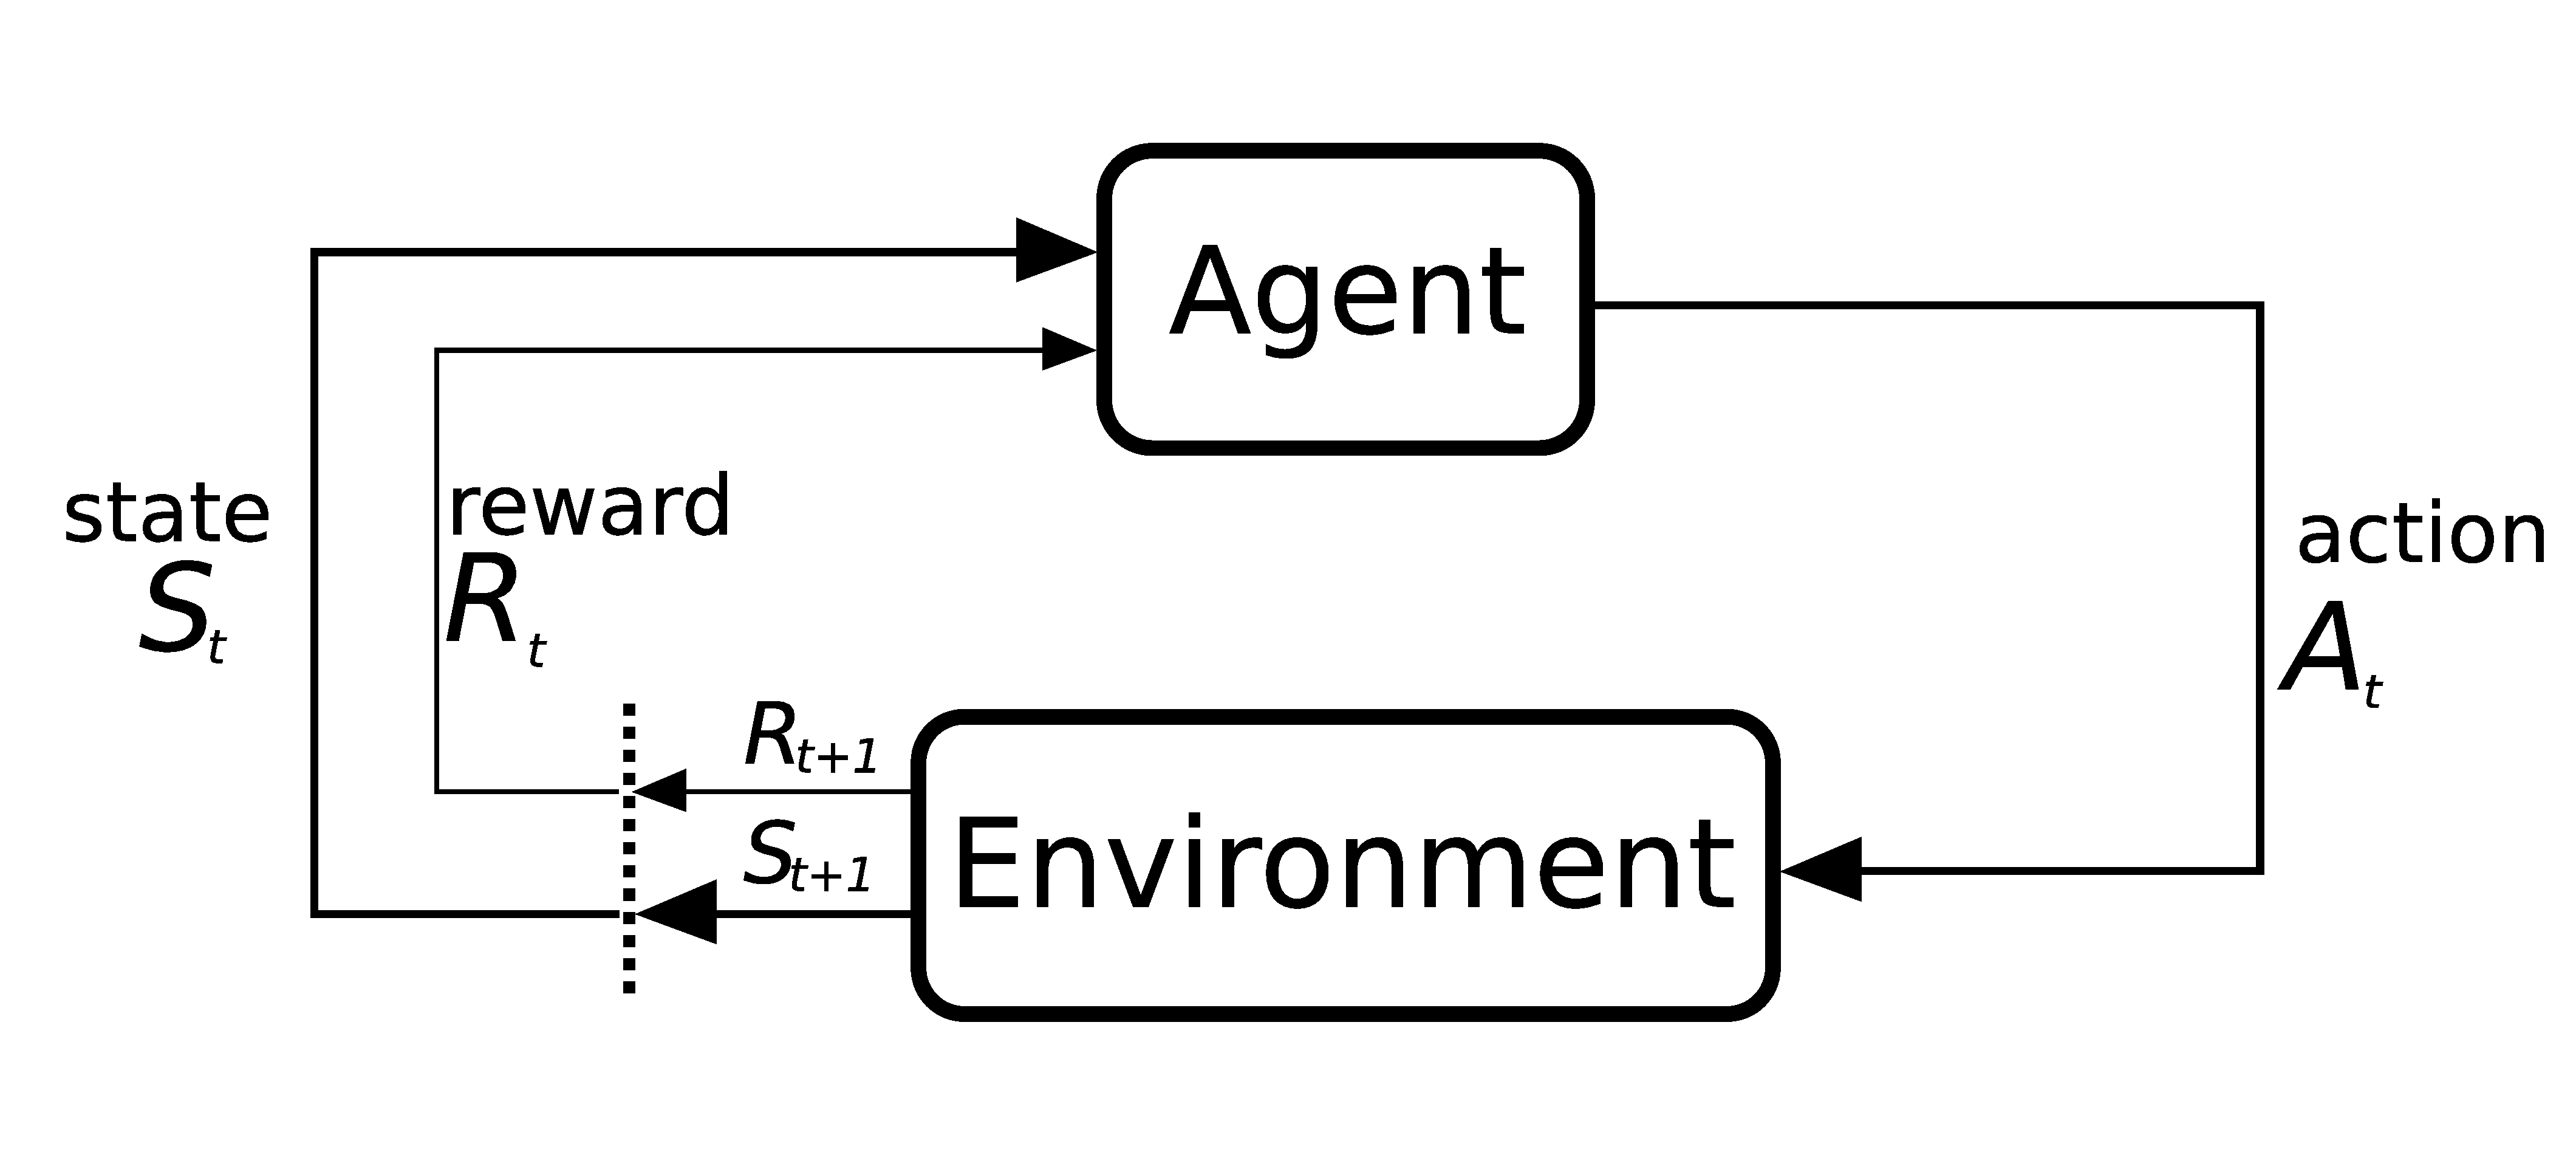
\includegraphics[scale=0.2]{Bilder/markov_diagram}
	\caption{Funktionsweise des Markov-Entscheidungsprozesses im Reinforcement Learning.}
	\label{fig.basics:rl:mdp}
\end{figure}

Die Entscheidung, welche Aktion in welchem Zustand ausgewählt wird, ist über die \textit{Policy} $\Pi_t$ des Agenten realisiert. $\Pi_t(a, s)$ ist dabei die Wahrscheinlichkeit, dass $A_t = a$, unter der Voraussetzung $S_t = s$. Vereinfacht ausgedrückt beschreibt $\Pi_t(a, s)$ damit die Wahrscheinlichkeit, dass zum Zeitpunkt $t$ im Zustand $s$ die Aktion $a$ gewählt wird.



\subsubsection{Markov-Eigenschaft}

Die Markov-Eigenschaft ist ein zentraler Bestandteil des \ac{MDP} und beschreibt 

\subsection{Bellman Gleichungen}

\section{}
\chapter{Organisation von Agenten}
\chapter{Kommunikationsstrategien}
\chapter{Lernalgorithmen}
\label{chap:learning}

Dieses Kapitel legt den Fokus primär auf die verschiedenen Lernalgorithmen und die zugrundeliegenden mathematischen Konzepte. Dazu werden zunächst in  Sektion \ref{chap:learning:single-agent} zwei wichtige Reinforcement Learning Algorithmen besprochen, die auf Umgebungen mit nur einem Agenten anwendbar sind. Zusätzlich wird eine Betrachtung durchgeführt, warum diese in der Theorie nur schlecht in Umgebungen mit mehreren Agenten einsetzbar sind. \\
Anschließend werden entsprechend modifizierte Algorithmen vorgestellt, die versuchen die benannten Probleme zu lösen bzw. entsprechend zu umgehen. 

\section{Single-Agent Anwendungsfall}
\label{chap:learning:single-agent}

\subsection{Q-Learning}

\subsection{Sarsa}

\subsection{Probleme für Multi-Agenten Systeme}

\section{Q-Learning}
\chapter{MAS Frameworks}
\chapter{Implementation einer Beispielanwendung}
\chapter{Fazit und Ausblick}

% ---- Literaturverzeichnis
\cleardoublepage
\renewcommand*{\chapterpagestyle}{plain}
\pagestyle{plain}
\pagenumbering{Roman}                   % Römische Seitenzahlen
\setcounter{page}{\numexpr\value{savepage}+1}
\printbibliography[title=Literaturverzeichnis]

% ---- Anhang
\appendix
%\clearpage
%\pagenumbering{Roman}  % römische Seitenzahlen für Anhang

\newpage
\end{document}
